\documentclass[../main/NEMO_manual]{subfiles}

\begin{document}

\chapter{North Pole Folding}
\label{apdx:NFOLD}

\chaptertoc

\paragraph{Changes record} ~\\

{\footnotesize
  \begin{tabularx}{\textwidth}{l||X|X}
    Release & Author(s) & Modifications \\
    \hline
    {\em   4.0} & {\em ...} & {\em ...} \\
    {\em   3.6} & {\em ...} & {\em ...} \\
    {\em   3.4} & {\em ...} & {\em ...} \\
    {\em <=3.4} & {\em ...} & {\em ...}
  \end{tabularx}
}

\clearpage

%% =================================================================================================
\section[North Pole Folding around a T-Point]{North Pole Folding around a T-Point}

When \forcode{l_Iperio = .true.}, \forcode{l_NFold = .true.} and \forcode{c_NFtype = 'T'} the North Pole Folding is done around 2 T-points. This is the case in ORCA 2\deg, 1/4\deg, 1/12\deg and 1/36\deg.

\begin{figure}[h]
  \centering
  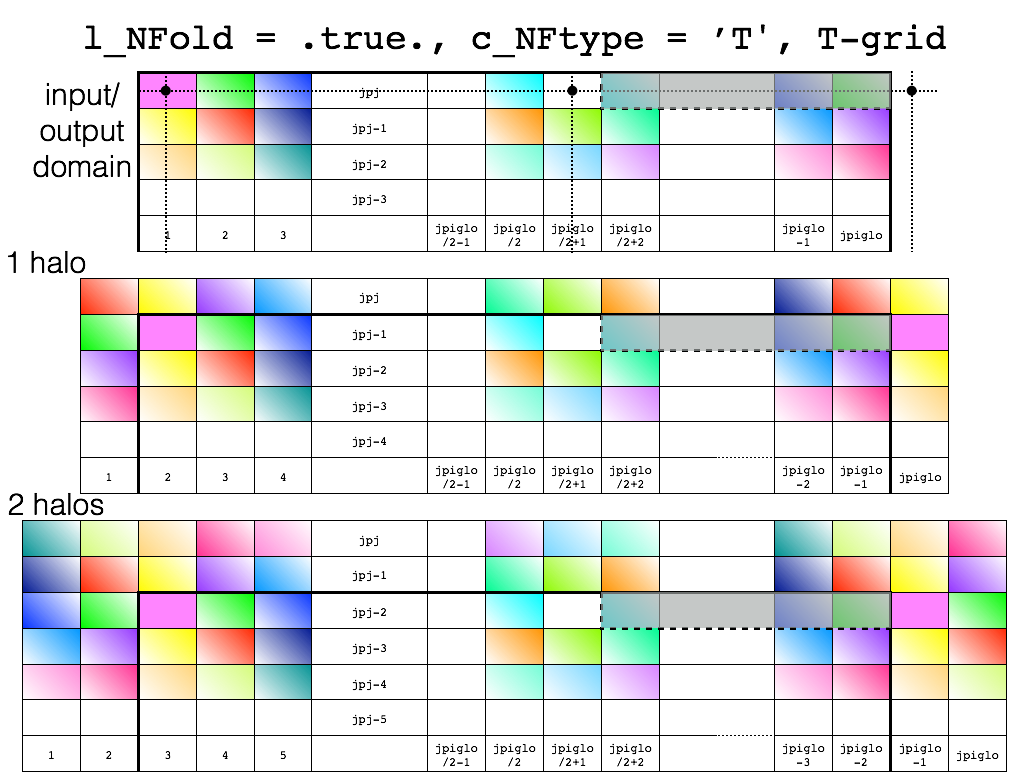
\includegraphics[width=0.9\textwidth]{NFT-T}
  \caption{
    North fold boundary for the T grid, with a $T$-point pivot and cyclic east-west boundary condition.
    Cells in the halos, outside of the inner domain (thick black line), will be defined by using only the values in the inner domain when calling the \rou{lbc\_lnk} routine (found in \mdl{lbclnk} module). Grey shading defines duplicated cells inside the inner domain that will also be refined (overwritten) by othe inner domain values when calling the \rou{lbc\_lnk}.
    Cells with the same color are at the same geographical location. Color shading shows the change in gradient on each side of the pivot-points.}
  \label{fig:NFT-T}
\end{figure}

\begin{figure}[t]
  \centering
  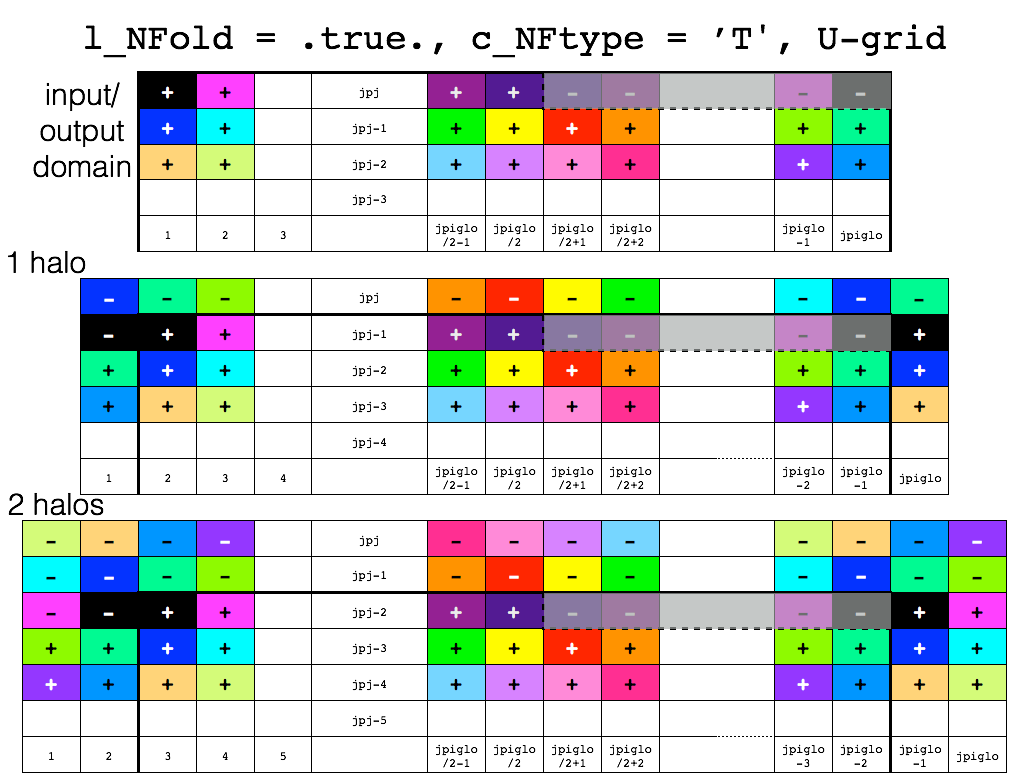
\includegraphics[width=0.9\textwidth]{NFT-U}
  \caption{
    North fold boundary for the U grid, with a $T$-point pivot and cyclic east-west boundary condition.
    Cells in the halos, outside of the inner domain (thick black line), will be defined by using only the values in the inner domain when calling the \rou{lbc\_lnk} routine (found in \mdl{lbclnk} module). Grey shading defines duplicated cells inside the inner domain that will also be refined (overwritten) by othe inner domain values when calling the \rou{lbc\_lnk}.
    Cells with the same color are at the same geographical location. Signs + or - are illustrating the change of signe on each side of the pivotal point.}
  \label{fig:NFT-U}
\end{figure}

\begin{figure}[t]
  \centering
  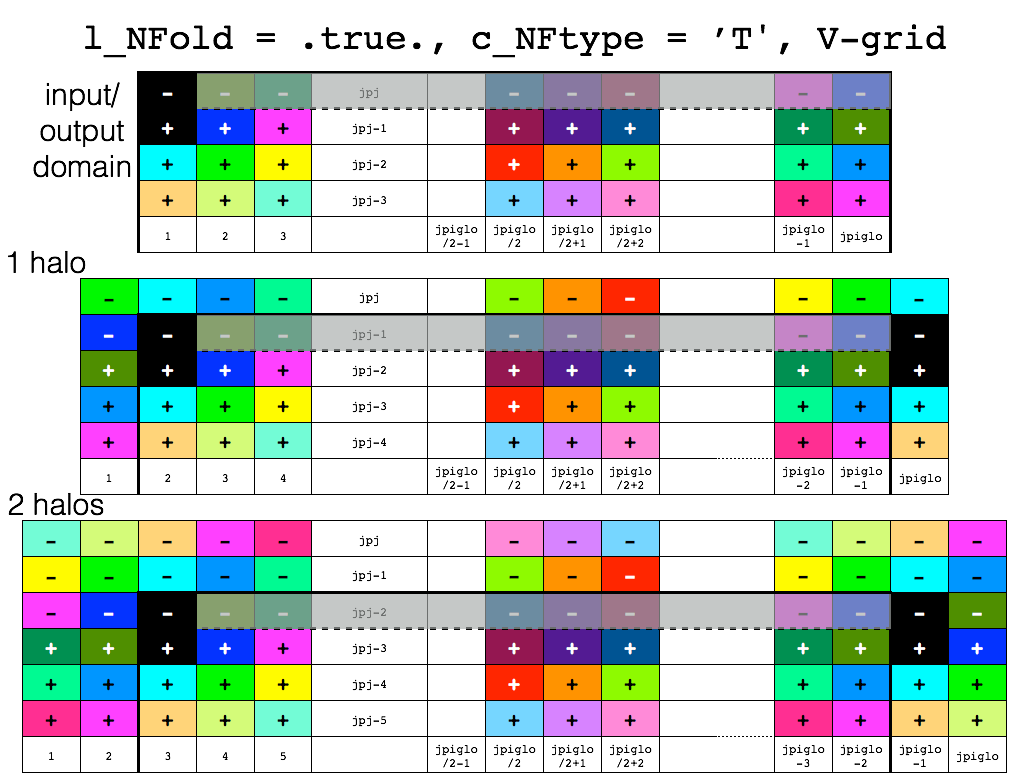
\includegraphics[width=0.9\textwidth]{NFT-V}
  \caption{
    North fold boundary for the V grid, with a $T$-point pivot and cyclic east-west boundary condition.
    Cells in the halos, outside of the inner domain (thick black line), will be defined by using only the values in the inner domain when calling the \rou{lbc\_lnk} routine (found in \mdl{lbclnk} module). Grey shading defines duplicated cells inside the inner domain that will also be refined (overwritten) by othe inner domain values when calling the \rou{lbc\_lnk}.
    Cells with the same color are at the same geographical location. Signs + or - are illustrating the change of signe on each side of the pivotal point.}
  \label{fig:NFT-V}
\end{figure}

\begin{figure}[t]
  \centering
  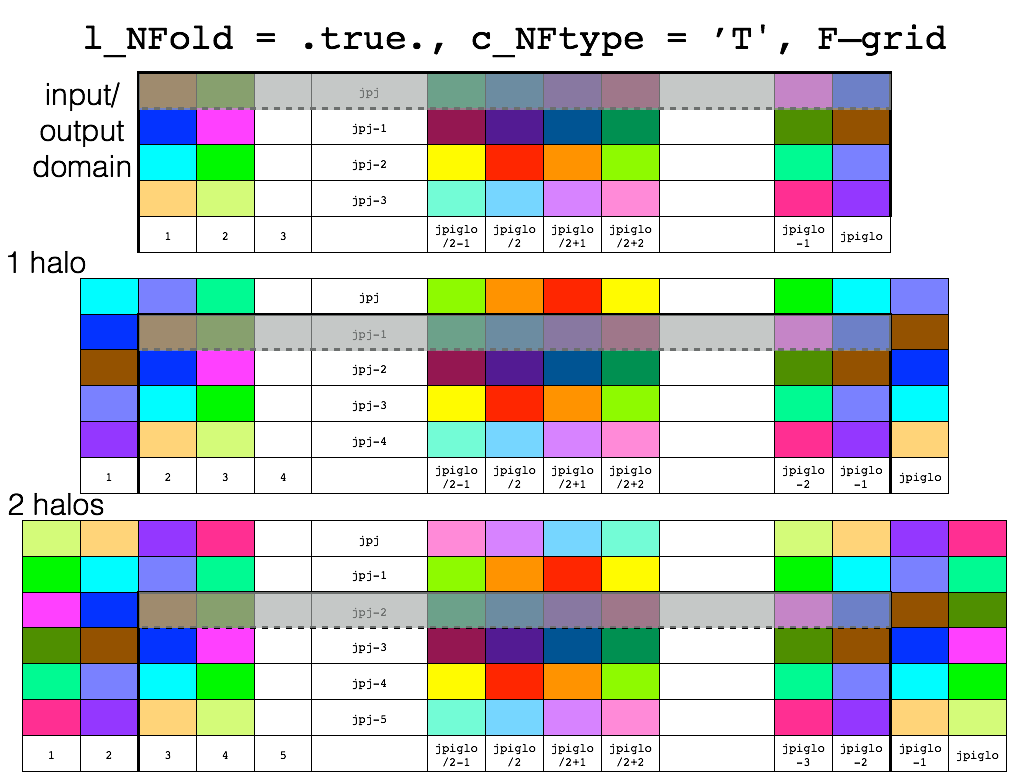
\includegraphics[width=0.9\textwidth]{NFT-F}
  \caption{
    North fold boundary for the F grid, with a $T$-point pivot and cyclic east-west boundary condition.
    Cells in the halos, outside of the inner domain (thick black line), will be defined by using only the values in the inner domain when calling the \rou{lbc\_lnk} routine (found in \mdl{lbclnk} module). Grey shading defines duplicated cells inside the inner domain that will also be refined (overwritten) by othe inner domain values when calling the \rou{lbc\_lnk}.
    Cells with the same color are at the same geographical location.}
  \label{fig:NFT-F}
\end{figure}

\clearpage

%% =================================================================================================
\section[North Pole Folding around a F-Point]{North Pole Folding around a F-Point}

When \forcode{l_Iperio = .true.}, \forcode{l_NFold = .true.} and \forcode{c_NFtype = 'F'} the North Pole Folding is done around 2 F-points. This is the case in ORCA 1\deg and 1/2\deg.


\begin{figure}[h]
  \centering
  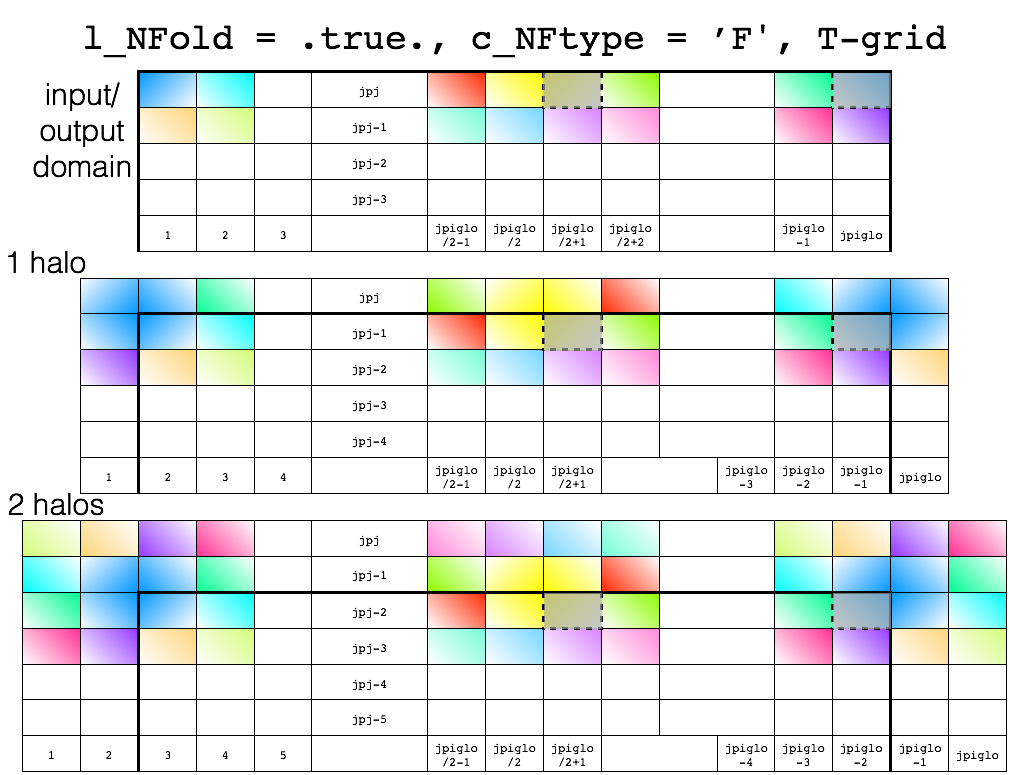
\includegraphics[width=0.9\textwidth]{NFF-T}
  \caption{
    North fold boundary for the T grid, with a $F$-point pivot and cyclic east-west boundary condition.
    Cells in the halos, outside of the inner domain (thick black line), will be defined by using only the values in the inner domain when calling the \rou{lbc\_lnk} routine (found in \mdl{lbclnk} module). Grey shading defines duplicated cells inside the inner domain that will also be refined (overwritten) by othe inner domain values when calling the \rou{lbc\_lnk}.
    Cells with the same color are at the same geographical location. Color shading shows the change in gradient on each side of the pivot-points.}
  \label{fig:NFF-T}
\end{figure}

\begin{figure}[t]
  \centering
  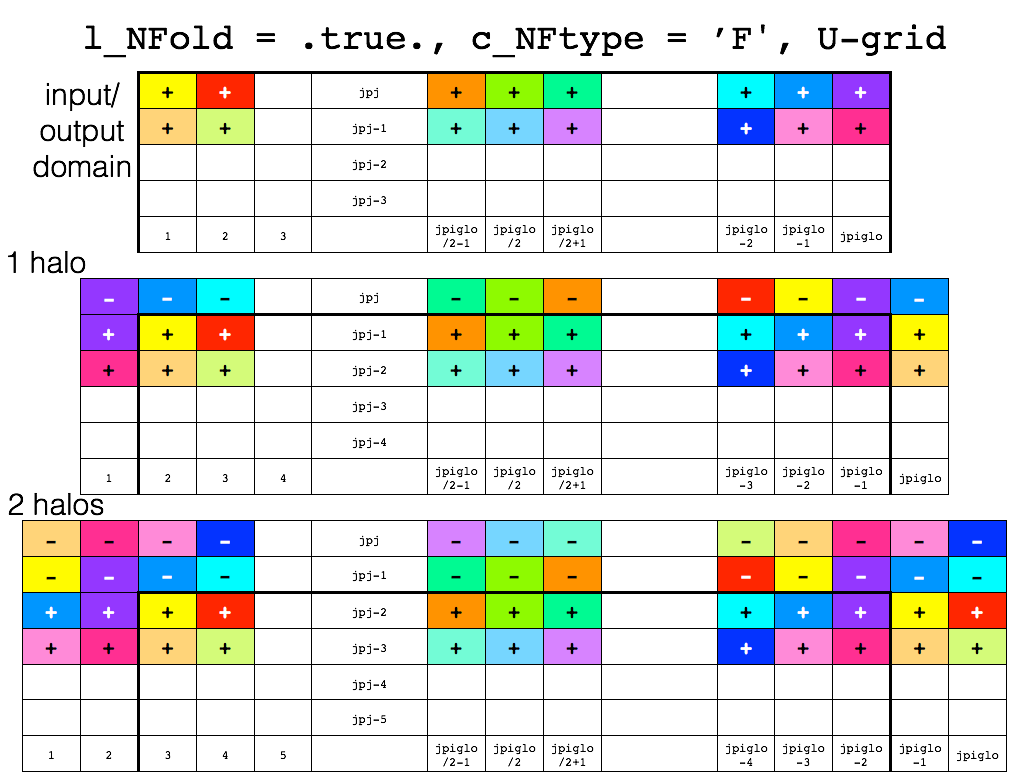
\includegraphics[width=0.9\textwidth]{NFF-U}
  \caption{
    North fold boundary for the U grid, with a $F$-point pivot and cyclic east-west boundary condition.
    Cells in the halos, outside of the inner domain (thick black line), will be defined by using only the values in the inner domain when calling the \rou{lbc\_lnk} routine (found in \mdl{lbclnk} module).
    Cells with the same color are at the same geographical location. Signs + or - are illustrating the change of signe on each side of the pivotal point.}
  \label{fig:NFF-U}
\end{figure}

\begin{figure}[t]
  \centering
  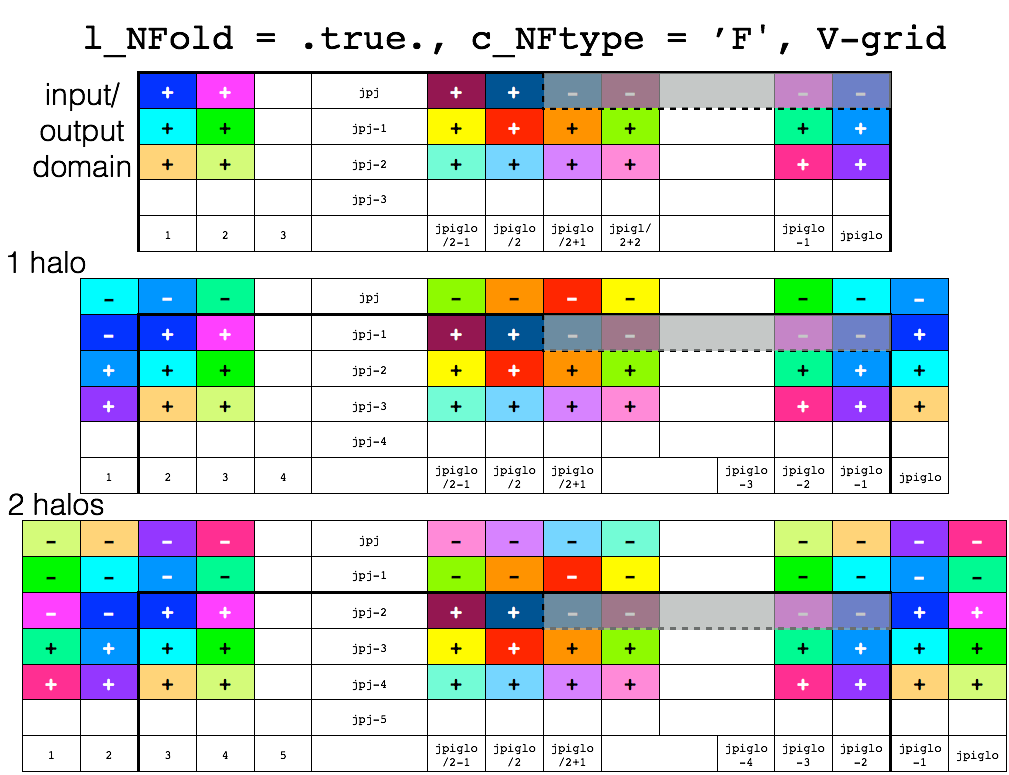
\includegraphics[width=0.9\textwidth]{NFF-V}
  \caption{
    North fold boundary for the V grid, with a $F$-point pivot and cyclic east-west boundary condition.
    Cells in the halos, outside of the inner domain (thick black line), will be defined by using only the values in the inner domain when calling the \rou{lbc\_lnk} routine (found in \mdl{lbclnk} module). Grey shading defines duplicated cells inside the inner domain that will also be refined (overwritten) by othe inner domain values when calling the \rou{lbc\_lnk}.
    Cells with the same color are at the same geographical location. Signs + or - are illustrating the change of signe on each side of the pivotal point.}
  \label{fig:NFF-V}
\end{figure}

\begin{figure}[t]
  \centering
  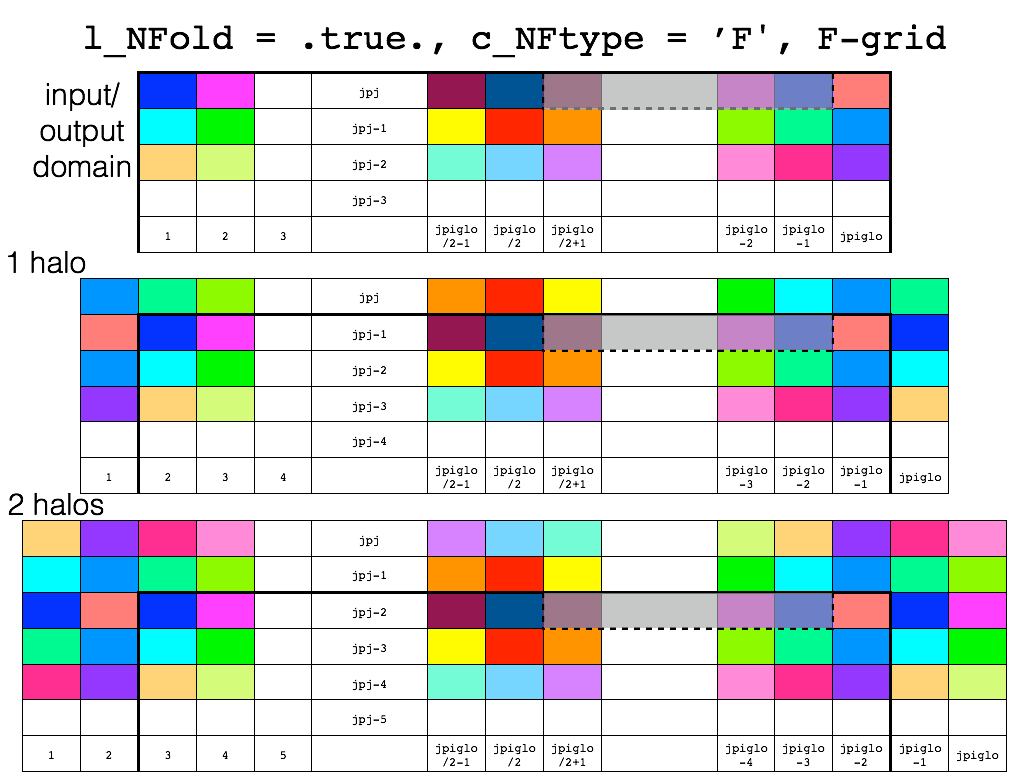
\includegraphics[width=0.9\textwidth]{NFF-F}
  \caption{
    North fold boundary for the F grid, with a $F$-point pivot and cyclic east-west boundary condition.
    Cells in the halos, outside of the inner domain (thick black line), will be defined by using only the values in the inner domain when calling the \rou{lbc\_lnk} routine (found in \mdl{lbclnk} module). Grey shading defines duplicated cells inside the inner domain that will also be refined (overwritten) by othe inner domain values when calling the \rou{lbc\_lnk}.
    Cells with the same color are at the same geographical location.}
  \label{fig:NFF-F}
\end{figure}


%% =================================================================================================
\subinc{%% =================================================================================================
%% Backmatter
%% =================================================================================================

%% Bibliography
%% =================================================================================================

\phantomsection
\addcontentsline{toc}{chapter}{Bibliography}
\lohead{Bibliography}
\rehead{Bibliography}
\bibliography{../main/bibliography}

\clearpage

%% Indices
%% =================================================================================================

\phantomsection
\addcontentsline{toc}{chapter}{Indices}
\lohead{Indices}
\rehead{Indices}
\printindex[blocks]
\printindex[keys]
\printindex[modules]
\printindex[parameters]
\printindex[subroutines]

\clearpage

%% Glossary
%% =================================================================================================

%\phantomsection
%\addcontentsline{toc}{chapter}{Glossary}
%\lohead{Glossary}\rehead{Glossary}
%\printglossaries
}

\end{document}
